\documentclass[]{book}
\usepackage{lmodern}
\usepackage{amssymb,amsmath}
\usepackage{ifxetex,ifluatex}
\usepackage{fixltx2e} % provides \textsubscript
\ifnum 0\ifxetex 1\fi\ifluatex 1\fi=0 % if pdftex
  \usepackage[T1]{fontenc}
  \usepackage[utf8]{inputenc}
\else % if luatex or xelatex
  \ifxetex
    \usepackage{mathspec}
  \else
    \usepackage{fontspec}
  \fi
  \defaultfontfeatures{Ligatures=TeX,Scale=MatchLowercase}
\fi
% use upquote if available, for straight quotes in verbatim environments
\IfFileExists{upquote.sty}{\usepackage{upquote}}{}
% use microtype if available
\IfFileExists{microtype.sty}{%
\usepackage[]{microtype}
\UseMicrotypeSet[protrusion]{basicmath} % disable protrusion for tt fonts
}{}
\PassOptionsToPackage{hyphens}{url} % url is loaded by hyperref
\usepackage[unicode=true]{hyperref}
\hypersetup{
            pdftitle={A Conditional Dinner},
            pdfauthor={A. Lucas},
            pdfborder={0 0 0},
            breaklinks=true}
\urlstyle{same}  % don't use monospace font for urls
\usepackage{natbib}
\bibliographystyle{apalike}
\usepackage{longtable,booktabs}
% Fix footnotes in tables (requires footnote package)
\IfFileExists{footnote.sty}{\usepackage{footnote}\makesavenoteenv{long table}}{}
\usepackage{graphicx,grffile}
\makeatletter
\def\maxwidth{\ifdim\Gin@nat@width>\linewidth\linewidth\else\Gin@nat@width\fi}
\def\maxheight{\ifdim\Gin@nat@height>\textheight\textheight\else\Gin@nat@height\fi}
\makeatother
% Scale images if necessary, so that they will not overflow the page
% margins by default, and it is still possible to overwrite the defaults
% using explicit options in \includegraphics[width, height, ...]{}
\setkeys{Gin}{width=\maxwidth,height=\maxheight,keepaspectratio}
\IfFileExists{parskip.sty}{%
\usepackage{parskip}
}{% else
\setlength{\parindent}{0pt}
\setlength{\parskip}{6pt plus 2pt minus 1pt}
}
\setlength{\emergencystretch}{3em}  % prevent overfull lines
\providecommand{\tightlist}{%
  \setlength{\itemsep}{0pt}\setlength{\parskip}{0pt}}
\setcounter{secnumdepth}{5}
% Redefines (sub)paragraphs to behave more like sections
\ifx\paragraph\undefined\else
\let\oldparagraph\paragraph
\renewcommand{\paragraph}[1]{\oldparagraph{#1}\mbox{}}
\fi
\ifx\subparagraph\undefined\else
\let\oldsubparagraph\subparagraph
\renewcommand{\subparagraph}[1]{\oldsubparagraph{#1}\mbox{}}
\fi

% set default figure placement to htbp
\makeatletter
\def\fps@figure{htbp}
\makeatother

\usepackage{booktabs}

\title{A Conditional Dinner}
\author{A. Lucas}
\date{2019-12-20}

\begin{document}
\maketitle

{
\setcounter{tocdepth}{1}
\tableofcontents
}
\chapter*{}\label{section}
\addcontentsline{toc}{chapter}{}

\begin{flushleft}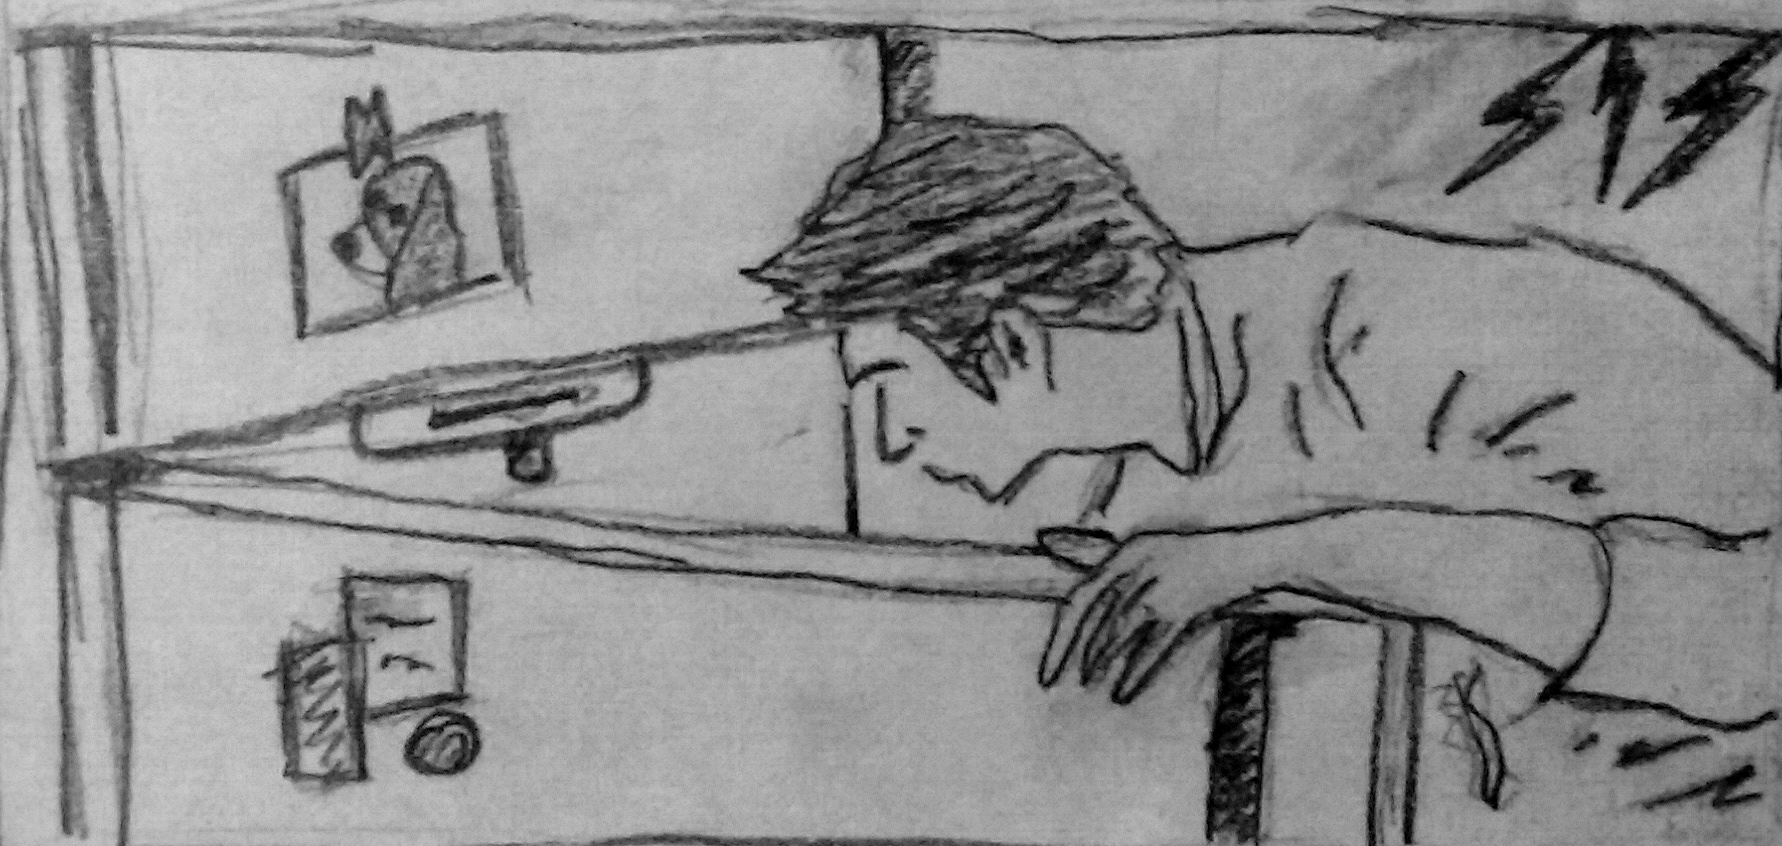
\includegraphics[width=0.5\linewidth]{images/titleimage} \end{flushleft}

\chapter{}\label{section-1}

I lifted my chin from my fist and looked at my watch. Seven twenty-two.
I tried to shift my weight on the hard, wooden bench in a futile effort
to relieve my bottom which had started to go numb, though it was
difficult as the five of us were practically on top of each other,
packed on it like sardines. We had gotten to the restaurant right on
time at seven o'clock and given our name to the hostess who had assured
us it would be a twenty minute wait at most. George had commented the
wait would be perfect since his wife, Kim, was always late anyway and
then made up some story about how they had come separately because he
had driven here straight from work. I knew perfectly well that was false
because my kitchen happened to be the perfect place for me to listen to
them fight for practically three weeks straight at every waking and
non-waking hour, including tonight right before Lisa and I had left for
the restaurant. Furthermore, some time ago as I was preparing a
particularly tasty pot roast for Lisa's and my anniversary, I found out
that George hadn't even had a job in upwards of three months because he
had gotten fired for stealing office supplies and ``stayed home all day
watching trashy daytime television yet couldn't even be bothered to have
dinner ready instead of applying for jobs.'' I had been so enthralled in
the dramatics, I completely lost track of time and was only reminded to
put the roast in the oven by the gnawing feeling in my stomach.

\chapter{}\label{section-2}

It was now seven thirty-four and my stomach seemed to grumble louder
each time a waitress came to seat another party, which would prompt a
new insult about Kim from George. I had eaten a sizable lunch for
someone with dinner plans, but for some reason I felt absolutely starved
sitting on that bench. Most of the time I was meant to be making Year
2000 date expansion software updates today at work had been spent
debating whether or not I would last long enough through the dinner to
make it to dessert so I could try the crème brûlée, but sitting there
with George buzzing in my ear, it was almost to the point that it was
all I could think about. I had heard co-workers raving about it on
several occasions and figured it was such an obscure dish for a
relatively downmarket restaurant to have as a specialty that it must be
particularly good. And sure enough, tray after tray of the most
exquisite looking crème brûlée I had ever laid eyes on was being served
to guest after guest as they finished their meals. I was honestly
surprised at how divine those little white dishes of custard looked as
the tacky mismatched decor and striped polo shirts did not exactly
scream ``Michelin star'' to me. I watched as the somewhat lanky, but
attractive couple seated closest to our bench took their first bites,
chewing with their mouths partially open to reveal little blobs of
cream, rolling their heads around their giraffe necks as their eyes
bulged out and making mouth noises. It should have repulsed me, but
instead it made it seem even more tempting.

\chapter{}\label{section-3}

Just then, in either an act of altruism or self-preservation, Dick
excused himself from George, who had gotten himself so worked up about
Kim he was now practically shouting as little beads of sweat formed on
his flushed brow, to inquire with the hostess how much longer it would
be. Thank God, because my stomach was really starting to develop its
voice.

\chapter{}\label{section-4}

``She said it would just be a few more minutes.''

I nodded gratefully at him, eyeing a fresh tray of crème brûlée. My
stomach growled so loudly, I thought it had startled George until I
realized he had only paused his latest rant to react to the little
coaster pager they had given us. I grabbed it from him in what even I
can admit was a somewhat hostile manner and took it up to the hostess.

``Party of six?''

I answered ``yes'' and gestured to my neighbors seated on the bench.

``Is everyone here? I only see five.''

``No, one person is running a little late.''

``I'm sorry, I can only seat full parties. If you let me know when she
gets here, we can get you situated or I can change the table to five.''

I have to say at this point I was fairly disgusted with the whole thing
and if not for that crème brûlée in the back of my mind, I would have
walked out of that restaurant right then dragging Lisa behind me. But
instead I walked back to the bench and explained in a tone that could
only be described as accusing that we won't be able to be seated until
Kim arrives, spurring several expletives from George who was looking
like a blotchy overfilled balloon that would burst at any moment. I'm no
doctor, but his blood pressure must have been through the roof. Dick and
Jane looked as if they wanted to shrink into oblivion and truthfully I
wished they would have just so I had more room on that bench. Something
had to make up for George's swelling.

\chapter{}\label{section-5}

It was only a moment later that Jane, as she was seated closest to the
door, announced that she saw Kim walking in. Lisa later denied it, but
I'm sure I saw her breathe a sigh of relief, grateful for a brief
intermission in the terribly detailed description of the plot of a novel
Jane was drafting, which sounded suspiciously similar to Pride and
Prejudice to the extent that it even featured a character named
Mr.~Darby. No sooner did Kim set one foot in the restaurant than George
immediately sprung up and began to accuse her of making everyone starve
to death. Before they could really get into it, Dick, who I was really
starting to come around to, announced that he would let the hostess know
everyone was here so we could be seated. I prayed that we would be so I
could appease my stomach, which now seemed to be competing with George's
roars.

\chapter{}\label{section-6}

I watched Dick all but plead with the hostess before he came back and
said that it would probably be another twenty minutes now. This caused
George and Kim to engage in a full fledged verbal brawl, drawing the
attention from almost everyone in the restaurant. By this time Lisa and
Jane had inched so far away from the bench they were practically in the
bug-eyed couple's booth and I had lost sight of Dick altogether. As I
scanned the room, I noticed a waitress just to my left staring at George
and Kim, completely ignoring the fresh tray of crème brûlée in her
hands. I was torn between flat out attacking her and retaining my front
row seat to the horrifically public airing of personal grievances. In
the span of roughly thirty seconds the whole restaurant had learned
about what a terrible cook Kim was and George's kleptomania and how Kim
should have known marrying George was a mistake ever since he had
cheaped out on the wedding. I was straining to hear about Kim's secret
lunch meeting with her high-school lover over what I would consider to
be my stomach's attempt to break the sound barrier when I saw the
hostess heading in our direction. The look in her eye said we were about
to be asked to leave and I saw my chance at that crème brûlée dwindling
with each step. Almost at the exact second Kim screamed that she wanted
a divorce, I pushed the hostess out of the way and lunged at the
waitress's tray, knocking both of us down in the process. I knew I
didn't have much time so I practically inhaled that sweet, sweet custard
using my bare hands as spoons. All of my commotion caused George and Kim
to stop screaming at each other long enough for everyone to direct their
attention to me. Without even looking, I felt another one of Lisa's
daggers hit me, only this time it was as if the deliciousness of the
crème brûlée was my shield, protecting me from her visual lashing. I'm
not sure if it was just because I was starving, but it really was the
best crème brûlée I ever had the pleasure of tasting.

\chapter{}\label{section-7}

The entire restaurant seemed to freeze for a minute not knowing how to
react until Dick walked back in and the hostess shouted at him that we
all needed to leave immediately. Somehow as the moving target poor Dick
had gotten the brunt of the hostess's wrath despite having missed all of
the drama unfolding. Kim miraculously managed to avoid it altogether as
she had stormed out at some point while I was sitting frozen on the
floor among all the other little dishes of custard from the waitress's
tray that had spilled over my pants. Lisa marched over and dragged me,
still covered in crème brûlée, out to the parking lot. The others
followed behind us- George beet red as ever, but now wheezing and
clutching his left arm, Jane looking like she had just witnessed a
murder, and Dick in a state of confusion having missed all of the
dramatics.

\chapter{}\label{section-8}

``What happened in there? I just went over to the burger place next door
to put our names in. They said it would be a twenty minute wait.''

\chapter{}\label{section-9}

George immediately declined, insisting he really should be getting home
as he unsteadily traipsed to his car before driving off, in the opposite
direction of the apartment building I might add. I had somehow been able
to stop myself from yelling after him that he really should be going to
get looked at instead, a feat of which I am still quite proud.
Surprisingly, Lisa said that we should probably be going, too, and
mumbled something to me about a ``Mrs.~Kennett'' under her breath. But
with the crème brûlée and excitement lining the bottom of my stomach
coupled with my newfound admiration for Dick, I rather animatedly tried
to convince her that waiting twenty minutes for a lousy burger was
genuinely the greatest idea I had ever heard. Not wanting to cause any
more of a scene, she reluctantly agreed on the condition that I
apologize to the Johnsons. A part of me did feel genuinely bad that the
rest of our party hadn't gotten a chance to have their way with that
crème brûlée and Jane in particular had been looking like she didn't
want to be anywhere within fifty feet of me, so I dutifylly expressed my
regret over my behavior and somehow persuaded them to continue our
evening. To tell the truth, I can be quite charismatic when I want to be
and once I mentioned that I had a line as the apothecary in my high
school's production of Romeo and Juliet, even Jane started to warm up to
me, and on that note, we four remaining party members headed into
Burgerland to again try our luck. I was sitting quite comfortably on the
cushioned (cushioned!) bench next to Lisa, who was blotting the crème
brûlée remnants on my pants with a tissue from her purse in a largely
unsuccessful attempt to erase her embarrassment and avoid Jane's
never-ending list of ideas for the screen adaptation of The Notebook,
which I'll admit were fairly amusing one way or another.

\chapter{}\label{section-10}

Miraculously, my hunger was even beginning to subside\ldots{} until I
spotted the bickering couple from the apartment upstairs and immediately
felt my stomach give a Pavlovian snarl.

\emph{A Conditional Dinner} was initially an exercise in attempting to
apply the idea of a bottle episode to a short story. Bottle episodes are
commonly used in television when budget constraints necesitate an
episode that is able to be produced cheaply or quickly, often meaning
the entire episode is restricted to a single set and core cast members.
Some famous examples include Friends' \emph{The One Where No One's
Ready}, Breaking Bad's \emph{Fly}, and Seinfeld's \emph{The Chinese
Restaurant}. An additional use of bottle episodes is to focus in on
characterization and explore traits and motives. I found this to
translate nicely to this piece, which is already placed under certain
constraints- a word bank, the length, and the requirement to create an
arc. To go along with the theme, I wanted the cast of characters to feel
like an ensemble that could be part of a sitcom yet be able to focus in
on the thoughts of one specific character, in this case our unnamed
narrator who serves as the ``Anchor'' comedic archetype. The inspiration
for the premise was the aforementioned Seinfeld episode, although any
other similarities are purely coincidental as I haven't seen the actual
episode. Stylistically I would say the piece was heavily influenced by
the first half of JD Salinger's \emph{Raise High the Roof Beam,
Carpenters}, in which an ecclectic cast of characters are sandwiched in
a car, stuck in traffic, in an attemp to make their way to a wedding
reception. I just couldn't resist a narrator that we want to dislike,
but deep down probably have more in common with than we'd like to admit.
In keeping with the sitcom-y feel, I wanted to make sure there were both
layered and overt jokes in the piece as well as some ``just a hair too
unrealistic for real life'' situations. As a reader or viewer, I like
having to work a little bit for a laugh as it makes me feel like I am in
on a private joke with the creators. It wasn't until after I finished
the first draft that I realized what I had actually created: a story
about a man who has spent so much time eavesdropping on his neighbors'
arguing from his kitchen, he has conditioned his stomach to react.

\bibliography{book.bib,packages.bib}

\end{document}
